\documentclass[12pt, a4paper, titlepage]{scrartcl}

\usepackage{lmodern}
\usepackage[utf8]{inputenc}
\usepackage[english]{babel}
\usepackage{graphicx}
\graphicspath{{./Figures/}}

\usepackage{url}
%\usepackage{titlesec}
%\newcommand{\sectionbreak}{\clearpage}
\usepackage{dirtree}
\usepackage{color}
\usepackage{listings}
\usepackage{caption}

%to get clickable links from table of contents
\usepackage{hyperref}
\hypersetup{
	colorlinks,
	citecolor=black,
	filecolor=black,
	linkcolor=black,
	urlcolor=black
}

%\pagestyle{myheadings}
%\markboth{ITI Seminar: Your Name}{ITI Seminar: Your Name}
\usepackage{fancyhdr}
\pagestyle{fancy}
\chead{}
\rhead{}
\lhead{\footnotesize Master Thesis: Institut für Softwaretechnologie - Software Engineering}
\lfoot{\footnotesize Ganesh Ramakrishnan} 
\rfoot{\footnotesize \thepage} 
\cfoot{}
\renewcommand{\headrulewidth}{0.4pt}
\renewcommand{\footrulewidth}{0.4pt}

\newcommand{\courierword}[1]{\textsf{\itshape #1}}{\fontfamily{pcr}\selectfont}%

\setlength{\parindent}{0.0cm}
\setlength{\parskip}{1ex}

\setkomafont{sectioning}{\normalcolor\bfseries}

\title{Continuous Integration in Space Avionics - A Design Using Declarative Build Automation Paradigms\\
\ \\
{\large Master Thesis \\
	Institut für Softwaretechnologie, \\
	Abteilung Software Engineering
\\
%Summer Term 2016
}
}

\author{Ganesh Ayalur Ramakrishnan  \\
  INFOTECH, Universität Stuttgart  \\
  \\
  Supervised by Johannes Lieder \\
  Examiner Prof. Dr. rer. nat. Stefan Wagner
}

%\date{Seminar talk given on \today} 
% \date{Seminar talk given on 25.05.2012}

\begin{document}
\maketitle
\tableofcontents 
\newpage

\section{Abstract}

\par There are several benefits when Continuous Integration (CI) is adopted for a software
development project. This provides for a mechanism to prevent human errors during
the build and test of the developed software, as well as help release the product on-time.
Other benefits include capturing errors before they start accumulating, easier integration
at defined intervals over the course of software development, and faster, comprehensive
feedback to developers. However, in an embedded domain, adopting CI is a challenging
activity. Binaries need to be cross compiled to different targets, extensive tool chain
arguments, various build configurations and performance issues especially in validation
testing and in static code analysis.
\par The existing literature provides little information to address the effect that the build
automation tools have on the design and implementation of a CI framework in an embedded
avionics domain. Tools like Make and Ant are primarily used for the build and
test stages of development. However, these tools do not inherently provide mechanisms
to integrate with CI tools. There is a need to design a framework to interface the build
system with a CI tool. This adds to the complexity of the project.
This thesis aims to design a CI workflow for an On-Board Software (OBSW) development
project. The study aims to bring out the challenges of using a conventional imperative
build approach during the set-up of a CI framework for the project. The proposal
is to adopt a build tool which is based on declarative build paradigms and provide
for mechanisms to easily integrate with CI tools. This study is as an action research
(AR) on employing an alternative build automation system with study results expressed
as quantitative or qualitative metrics. A prototypical CI chain will be implemented
with a Jenkins CI server and Gradle as the primary build tool. Parameters such as
performance, maintenance complexity of build logic, reproducibility of builds are some
of the parameters under study.

\section{Introduction}

\section{Background and Research Approach}

\subsection{Background}
\subsubsection{Continuous Integration}
\subsubsection{Build Systems}
\par This section attempts to describe in brief about the build systems which are used in the project under study. A more detailed analysis of the build logic in the Make based and Gradle based build systems would be discussed later. 
\paragraph{Make}
\par Make is a popular build automation tool which is responsible for creating an executable or a library from source code. It manages to do this by parsing a file called Makefile. Software Development of the Make tool started more than 35 years ago\cite{Feldman1979} and there are several variants that are currently available. A very popular and widely used variant is the GNU Make. The format of the Makefiles are similar to one shown below\cite{GNUMakeManual}. 

\noindent\fbox{%
	\parbox{\textwidth}{%
	target : prerequisites \\
		 \hspace{10mm} recipe
	}%
}



\paragraph{Ant}
\paragraph{Gradle}

\subsection{Research Approach}
\subsubsection{Action Research}
\subsubsection{Qualitative Metrics in Study}


\section{On-Board Software Development (OBSW) - AS400 Central Software (CSW)}
The case organization chosen for this study is the Space Systems satellite On-Board Software Development (OBSW) department at Airbus Defence and Space, Friedrichshafen. This chapter provides an overview of the Software Development activities for AS400 Central Flight Software (CSW) as well as a description of the existing Software Development Environment (SDE) for the same.
\subsection{Overview}
The actual software that runs in an On Board Computer (OBC) in a satellite in operation is the On Board Software (OBSW). The OBSW is treated as isolated and independent software controlling the various applications such as power systems, propulsions, sensors and payload on a satellite. The AS400 Avionics development is an initiative towards a detailed definition and development of a generic, re-usable high power avionics system to be used on a variety of missions. 

\subsection{Software Development Environment (SDE)}
\par The team for AS400 Central Flight Software (CSW) is composed of two groups. A production team which provides the flight code and a validation team which performs the validation activities on the provided flight code. The production flight code is in C and the validation test framework is in Java. The SDE that is used by these teams is also composed of two parts. A client side SDE used by developers which consists of development packages in a Windows/Cygwin environment with Eclipse TOPCASED.  And a server side SDE consisting of the Atlassian Tool Suite (JIRA, Stash, Confluence, FishEye, Crucible) [?]. 
\par As with many embedded applications, this software system is also developed in a cross development environment\cite{rtemsIntro}. The existing SDE set-up utilizes GNU Make\cite{GNUMakeManual} as the build automation tool and GNU cross compilation tools for the project specific target space processors on the host systems. On the server side, JIRA is used for issue tracking and project management, Confluence for team collaboration, Bitbucket (formerly Stash) as repository management tool and Crucible for code review. The version control system used is Git\cite{GitflowWorkflow}. 
Figure~\ref{fig:sde-chart} shows an overview of the SDE used in this project. The blue lines indicate the links between the various applications. The straight black arrows indicate the interface between the team members and the SDE. The dotted arrows and the blocks in red are introduced as part of this thesis. As part of this study, the tools which will be integrated to the existing system are Jenkins and Gradle. Jenkins is an open source automation server which is used for continuous integration. An instance of Jenkins runs on the same server which also caters to the Atlassian Tool Suite. This instance is called as the Jenkins Master instance. The actual build steps are done on so called Slave Machines which are separate Linux based virtual machines. Gradle is the build automation tool under study which is installed on the Linux based machines as it is here where the build processes are expected to run.

\begin{figure}[!ht]
\centering
\caption{SDE set-up for AS400 Central Software Development}
\label{fig:sde-chart}
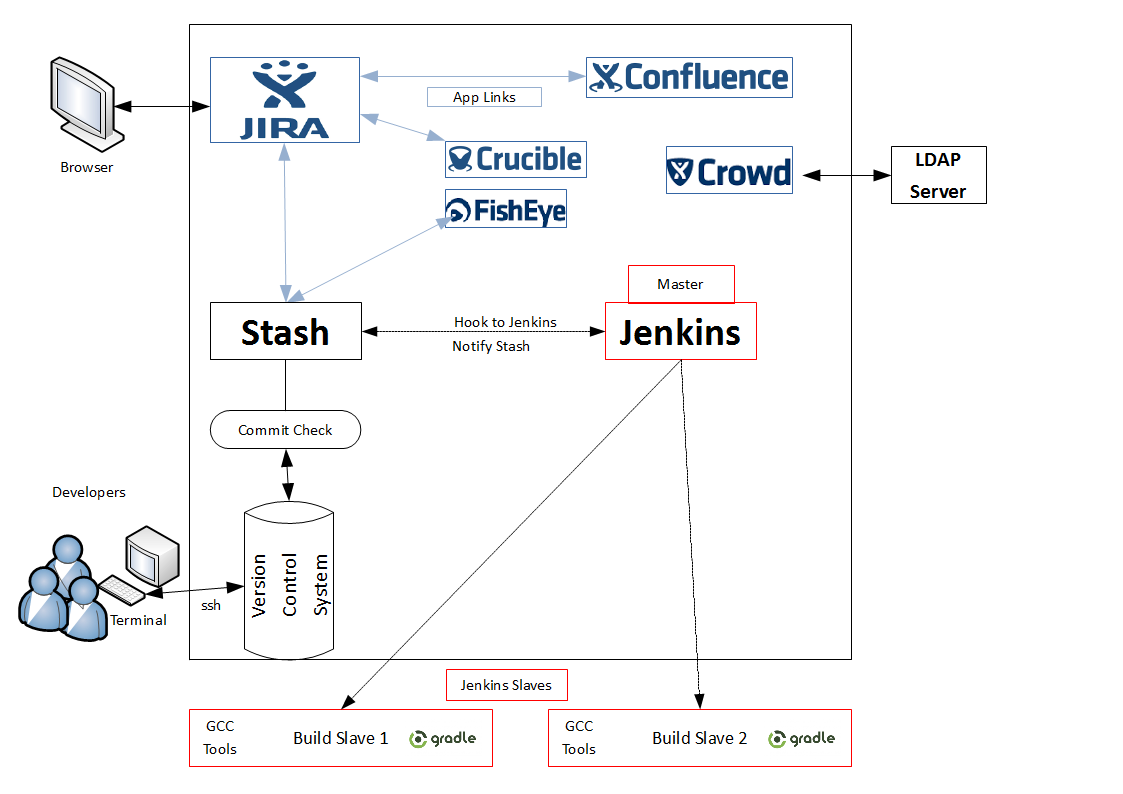
\includegraphics[width=\textwidth,height=\textheight,keepaspectratio]{SDE-Chart.png}
\end{figure}

\subsection{Software Development in OBSW - CSW}
This section explains the project specific terminology, structure of the source code, git workflow and the build automation methodology employed.
\subsubsection{Terminology}
The source code for the AS400 CSW development is organized as a hierarchy. There are five levels of elements. The top most level is the production repository. The second level contains the different aspects of production such as SDE scripts, source code, and libraries to be used in unit testing. The definition of the levels below this need to be distinguished using a view model. This study defines two distinct view models for the hierarchy. They are the Developer's view model and the Build Author's view model. \\
\\
\textbf{Developer's View Model}
\begin{itemize}
	\item Applications - they are elements which implement functional processing that are associated with the satellite. Some examples include Data Management System (DMS) which implements data handling standards, and Attitude and Orbit Control Systems (AOCS) which maintains the orientation of the satellite.
	\item Components - Applications can be composed of smaller entities called components. <fill-up-about-constituents>
\end{itemize}
\textbf{Build Author's View Model}
\begin{itemize}
	\item Collections - The elements which are at the same level within the flight software (fsw) folder in the hierarchy are called Collections. 
	\item Constituents - Subordinates of collections which generally contain the source files are called constituents. They usually build up to give the notion of an Application. It is common that some constituents contain further sub-constituents.
\end{itemize}
It should also be noted that Collections do not necessarily map directly towards Applications. 

\subsubsection{AS400 CSW Architecture }
As mentioned, the AS400 Project consists of several repositories. Figure~\ref{fig:as400-top-level} shows the various repositories that are used in this stufy. There are dedicated repositories for production (as400prod) and Validation (as400val). There is also a repository which contains the Make based build logic that is common for the project, as well as SDE tool interfaces such as for Static Code Analysis and Unit Testing. The scripts repositories contain the Glue Logic which creates the interface between the build tools and the CI tools. In addition it contains some helper scripts which allow for integration with Jenkins server. The hierarchy of the production repository is similar to the code tree shown in Figure~\ref{fig:prod-repo-structure}. Some of the Collections within these repositories are git submodules\cite{chacon2011git}.  

\begin{figure}[h]
\caption{The AS400 Project top level view.}
\label{fig:as400-top-level}
\noindent\fbox{%
\parbox{\textwidth}{%
\dirtree{%
.1 AS400 Project.
.2 as400prod	-------- Production Repository.
.2 as400val		-------- Validation Repository.      
.2 rtems		-------- RTEMS Operating Systems libraries for link.
.2 SDE			-------- Common Build Logic + SDE Tools.
.2 scripts		-------- Glue Logic for Jenkins, helper scripts, \dots.
}
}%
}
\end{figure}
\begin{figure}
\caption{An excerpt of the AS400 Production Repository Structure}
\label{fig:prod-repo-structure}
\noindent\fbox{%
\parbox{\textwidth}{%
\dirtree{%
.1 as400prod.
.2 delivery.
.2 fsw.
.3 aocs           -------------Collection Level.
.4 \color{blue}aocs.          
.4 \color{blue}aocsEquipments -------------Constituent Level.
.5 cbh            -------------Sub-Constituent Level.
.5 str.
.4 \color{blue}aocsMcl.
.3 asw.
.3 boot.
.3 \color{red}dms.
.3 \color{red}infra.
.2 \color{red}sde\_config.
.2 usvf.
.2 uml.
}
}%
}
\end{figure}
\par The folders in red are git submodules. The folders in blue are Constituents. The sub-directories within the folder fsw are Collections. This is only an excerpt of the original structure. The actual code tree consists of a larger number of Collections and Constituents. Collections may or may not contain Constituents. The production repository as viewed from the top level of the AS400 Project is self contained. 
\subsection{Software Development Workflow}
The AS400 CSW team employs a Gitflow Workflow\cite{GitflowWorkflow} for software development. There are five different types of branches – \courierword{master, develop, release, feature} and \courierword{bugfix} branches. \courierword{master} contains the official release history, integration of the features are done on \courierword{develop}, and the \courierword{feature} and \courierword{bugfix} branches are used primarily by the developers to work on individual collections. Just ahead of a software release, a new branch called \courierword{release} is forked off from \courierword{develop}. <add functionality of release here> When it is ideal for a release, it is merged with the \courierword{master}.   

\subsection{Build Automation in AS400 CSW}
This section describes in detail the tools and the methodology behind the builds in AS400. In the production environment, the builds for this project are done using GNU Make. In validation, the builds are done within the Eclipse IDE. However, as a headless framework is required for running the builds on remote machines, Apache Ant is used as the build tool. For compilation and linking, GCC tools (part of GNU software) for usage with the RTEMS operating system are used. For Java sources, an eclipse java compiler is used. 
The build system used in the AS400 Project is an inherited system. It has been used previously on successful software projects developed on similar platforms. 
\par The next part of this section describes the build logic employed to compile and link the production sources into respective binaries at different points during the build stage. The sources are compiled using Makefiles which are defined in each directory within the source code tree. There are also several ‘common’ Makefiles which define variables and rules. The build system uses a recursive Make model.   
Essentially, the CSW is to be delivered as an executable file. To achieve this goal, the build system uses the technique of Partial Linking [?]. This is explained with the help of an example. 
Assume we are considering the AOCS collection in the source tree. It is represented in Figure~\ref{fig:source-tree-collection-constituent}. Also Figure shows contents of the Makefiles at Collection and Constituent Levels.
\begin{figure}[!ht]
\caption{Source Tree of one of the Collections containing Constituents and Sub-Constituents}
\label{fig:source-tree-collection-constituent}
\noindent\fbox{%
\parbox{\textwidth}{%
\dirtree{%
.1 aocs.
.2 aocs.
.3 \color{red}Makefile.
.3 source.c.
.3 header.h.
.2 aocsApFw.
.3 \color{red}Makefile.
.3 source.c.
.3 header.h.
.2 aocsEquipments.
.3 cbh.
.4 \color{red}Makefile.
.4 source.c.
.4 header.h.
.3 gnss.
.4 \color{red}Makefile.
.4 source.c.
.4 header.h.
.3 mag.
.4 \color{red}Makefile.
.4 source.c.
.4 header.h.
.3 mtq.
.4 \color{red}Makefile.
.4 source.c.
.4 header.h.
.3 \color{red}Makefile.
.2 aocsMcl.
.3 \color{red}Makefile.
.3 source.c.
.3 header.h.
.2 aocsMclIf.
.3 \color{red}Makefile.
.3 source.c.
.3 header.h.
.2 \color{blue}Makefile.
}
}%
}
\end{figure}

\begin{figure}[!ht]
\caption{Makefile for 'aocs' Collection}
\label{fig:makefile-aocs}
\lstset{language=make,
		commentstyle=\color{red},
    	breaklines=true,
    	basicstyle=\scriptsize
}
\begin{lstlisting}[frame=single][t]
DEFAULT_MAKE = linkpart

# EXTERNAL_LIB : Definition of libraries to use for link, either local to the
#                directory or distant
EXTERNAL_LIB = lib/libaocsApFw.o \
               lib/libaocs.o \
               lib/libaocsEquipments.o \
               lib/libaocsMclIf.o \
               lib/libaocsMcl.o \

LIBDIR = $(OBSW_PATH)/lib

# EXTERNAL_LIB_INST : Definition of libraries to use for link in instrumented mode, either local to the
#                directory or distant
EXTERNAL_LIB_INST =  libaocsApFw.o \
                     libaocs.o \
                     libaocsEquipments.o \
                     libaocsMclIf.o \
                     libaocsMcl.o \
               
# INCLUDE OF GLOBAL RULES
#------------------------
include $(CPL_REP_MAKE)/Make.rules
\end{lstlisting}
\end{figure}
\begin{figure}[!ht]
\caption{Makefile for 'aocsApFw' Constituent}
\label{fig:makefile-aocsApFw}
\lstset{language=make,
		commentstyle=\color{red},
    	breaklines=true,
		basicstyle=\scriptsize    	
}
\begin{lstlisting}[frame=single][t]
DEFAULT_MAKE = linkpart

EXTRA_INCLUDE = -I$(AOCS_PATH)/aocsEquipments \
                -I$(AOCS_PATH) \
                -I$(DHS_PATH) \
                -I$(INFRA_PATH) \
                -I$(IO_PATH)/busMgr \
                -I$(IO_PATH)/busCplr \
                -I$(IO_PATH)/pmCplr \
                -I$(IO_PATH)/rmapCplr

# SRC : Definition of sources to compile
SRC = AocsApFw.c \
      AocsSync.c \
      AocsAsync.c 

EXTRA_CLEAN = AocsApFwParam.c

# INCLUDE OF GLOBAL RULES
#------------------------
include $(CPL_REP_MAKE)/Make.rules
\end{lstlisting}
\end{figure}
There are Makefiles within each Constituent and Sub-Constituent directories (in red) as well as within the Collection (in blue). The Makefiles at Collection level and Constituent levels are shown in the Figures~\ref{fig:makefile-aocs} and~\ref{fig:makefile-aocsApFw} . 
\par Initially, the sources within the Constituent and Sub-Constituent directories are compiled. This is followed by the first stage of link where only partial linking is done. A single relocatable output file is produced which can be used as an input file for later link stages. Partial linking is achieved by use of the appropriate linker arguments. Each of the Constituents produces one partially linked object file. The Makefile at the Collection level does the second stage of link. Here all the object files produced at its Constituent level are partially linked. For Constituents which have Sub-Constituents, for example the aocsEquipments Constituent, there is partial linking at the Sub-Constituent stage and then a secondary partial link stage at the Constituent level. This behaviour is common for all Collections and Constituents throughout the source code tree. The build process is so designed that the output of every partial link stage gives rise to an object file which is stored at a level higher than the directory in which the linkpart target is executed. One feature of partial linking is that the unresolved references remain unresolved. At the time of generating the complete CSW executable, there is a final link stage where all the partially linked objects of the different collections are linked together to produce the software executable. In addition to the partially linked object and the executable, the build system also provides for building a static library from the sources. Some of these libraries are used at the final link time to resolve references. 
\par The build system also provides for building two different variants of the image. The variants differ primarily in the way the sources are compiled. The project defines two distinct database exports which contain several ‘\#define’ directives for many identifiers used within the source codes. These image variants are called the SYSDB (system database) and SWDB (software database). The build system allows for generation of these variants based on a command line property. 
\par The project also defines two other variants based on the platform for which the sources are compiled. They are the SCOC3\cite{koebel2010scoc3} and native PC. It should be noted that not all sources in the tree can be compiled for PC. A good example is the 'startup' Collection which contains assembler sources. Hence, the notion of a complete CSW executable for a PC does not exist. However, in the realm of Unit Testing, the compilation for PC platform is  important for capturing bugs. For producing variants depending on the platform, different tool chains are used. For SCOC3, the GNU sparc-rtems compiler and linker are used while for PC the native GNU compiler and linker packages are used. The existing build systems allows for generation of these variants also based on a command line property.
\par Now, let us analyze the Makefiles in Figures~\ref{fig:makefile-aocs} and~\ref{fig:makefile-aocsApFw} . Each of these Makefiles includes the ‘common’ Makefile which is called Make.rules. It is like a root Makefile which defines and describes the targets used in these Makefiles. As shown in the figure 'linkpart' is the default target in both these Makefiles. The activity carried out in these Makefiles is partial linking. In the Constituent's Makefile, the variable SRC determines the sources that need to be built. The EXTRA\_INCLUDE variable adds a set of paths which the compiler traverses through to find the include headers for the sources. In the Makefile at Collections level, the EXTERNAL\_LIB variable defines various partially linked objects which need to be sources to the linker. The LIBDIR variable defines the directory to which the output of the link process would be written to.


\section{Gradle for AS400 CSW}
 This section aims to define the Gradle model which is developed for the software development project under study. 
\subsection{Terminology}
\subsection{Build System Design Aspects}
\subsection{Analysis of Build Logic}

\section{Continuous Integration in AS400 CSW}
\subsection{Terminology}
\subsection{CI Workflow for AS400 CSW}
\subsection{Challenges faced during design}

\section{Evaluation and Results}
\subsection{Performance Comparison}
\subsection{Complexity of Build Logic}
\subsection{Feature Comparison}
\subsection{Summary}

\section{Conclusion}
\subsection{Summary}
\subsection{Future Work}


%\section{Summary}\label{sec:Summary}

%This report focussed on \ldots


\bibliographystyle{ieeetr}
\bibliography{seminar-template} % uses the seminar-template.bib file as input

\end{document}

